%\documentclass[final,hyperref={pdfpagelabels=false},unknownkeysallowed]{beamer}
\pdfminorversion=4
\documentclass[xcolor=dvipsnames]{beamer}



%Load the myriad packages
\usepackage{xcolor}
\usepackage{subcaption}
\usepackage{tikz}
\usetikzlibrary{shapes.geometric, arrows}
\tikzstyle{startstop} = [rectangle, rounded corners, minimum width=2cm, text
    width=1.8cm, minimum height=1cm,text centered, text=white,draw=black, fill=Gray!140]
\tikzstyle{io} = [trapezium, trapezium left angle=70, trapezium right angle=110,
minimum width=0.5cm, minimum height=1cm, text centered, draw=black,
fill=blue!20!Gray!90!,text=white]
\tikzstyle{process} = [rectangle, minimum width=2cm, minimum height=1cm, text
centered, text width=2cm, draw=black, text=white,fill=Gray!140!blue!70!white]
\tikzstyle{decision} = [diamond, minimum width=2.0cm, minimum
    height=0.81cm,aspect=1.40, text centered, draw=black, fill=Gray!,text=white]
\tikzstyle{arrow} = [thick,line width=0.5mm,->,>=stealth]
\tikzstyle{arrow1} = [dashed,->,>=stealth]

%
% Ways of grouping things
%
\newcommand{\bracket}[1]{\left[ #1 \right]}
\newcommand{\bracet}[1]{\left\{ #1 \right\}}
\newcommand{\fn}[1]{\left( #1 \right)}
\newcommand{\ave}[1]{\left\langle #1 \right\rangle}
\newcommand{\norm}[1]{\Arrowvert #1 \Arrowvert}
\newcommand{\abs}[1]{\arrowvert #1 \arrowvert}

%
% Derivative forms
%
\newcommand{\dx}[1]{\,d#1}
\newcommand{\dxdy}[2]{\frac{\partial #1}{\partial #2}}
\newcommand{\dxy}[2]{\frac{d #1}{d #2}}
\newcommand{\dxdt}[1]{\frac{\partial #1}{\partial t}}
\newcommand{\dxdz}[1]{\frac{\partial #1}{\partial z}}
\newcommand{\dfdt}[1]{\frac{\partial}{\partial t} \fn{#1}}
\newcommand{\dfdz}[1]{\frac{\partial}{\partial z} \fn{#1}}
\newcommand{\ddt}[1]{\frac{\partial}{\partial t} #1}
\newcommand{\ddz}[1]{\frac{\partial}{\partial z} #1}
\newcommand{\dd}[2]{\frac{\partial}{\partial #1} #2}
\newcommand{\ddx}[1]{\frac{\partial}{\partial x} #1}
\newcommand{\ddy}[1]{\frac{\partial}{\partial y} #1}
\newcommand{\dxdyn}[3]{\frac{\partial ^{#3} #1 }{\partial #2 ^{#3}}}
\newcommand{\Dxdy}[2]{\frac{D #1}{D #2}}
\newcommand{\Dxy}[2]{\frac{D #1}{D #2}}
%
% Vector forms
%
\renewcommand{\vec}[1]{\mbox{$\stackrel{\longrightarrow}{#1}$}}
\renewcommand{\div}{\mbox{$\vec{\nabla} \cdot$}}
\newcommand{\grad}{\mbox{$\vec{\nabla}$}}
\newcommand{\bb}[1]{\bar{\bar{#1}}}
%
% Equation beginnings and endings
%
\newcommand{\bea}{\begin{eqnarray}}
\newcommand{\eea}{\end{eqnarray}}
\newcommand{\be}{\begin{equation}}
\newcommand{\ee}{\end{equation}}
\newcommand{\beas}{\begin{eqnarray*}}
\newcommand{\eeas}{\end{eqnarray*}}
\newcommand{\bdm}{\begin{displaymath}}
\newcommand{\edm}{\end{displaymath}}
%
% Equation punctuation
%
\newcommand{\pec}{\, ,}
\newcommand{\pep}{\, .} 
\newcommand{\pev}{\hspace{0.25in}}
%
% Equation labels and references, figure references, table references
%
\newcommand{\LEQ}[1]{\label{eq:#1}}
\newcommand{\EQ}[1]{Eq.~(\ref{eq:#1})}
\newcommand{\REQ}[1]{\ref{eq:#1}}
\newcommand{\LFI}[1]{\label{fi:#1}}
\newcommand{\FI}[1]{Fig.~\ref{fi:#1}}
\newcommand{\RFI}[1]{\ref{fi:#1}}
\newcommand{\LTA}[1]{\label{ta:#1}}
\newcommand{\TA}[1]{Table~\ref{ta:#1}}
\newcommand{\RTA}[1]{\ref{ta:#1}}
\newcommand{\lequ}[1]{\label{eq:#1}}
\newcommand{\equ}[1]{Eq.~(\ref{eq:#1})}
\newcommand{\equs}[1]{Eqs.~(\ref{eq:#1})}
\newcommand{\requ}[1]{(\ref{eq:#1})}
\newcommand{\lfig}[1]{\label{fi:#1}}
\newcommand{\fig}[1]{Fig.~\ref{fi:#1}}
\newcommand{\figs}[1]{Figs.~\ref{fi:#1}}
\newcommand{\rfig}[1]{\ref{fi:#1}}
\newcommand{\lta}[1]{\label{ta:#1}}
\newcommand{\ta}[1]{Table~\ref{ta:#1}}
\newcommand{\rta}[1]{\ref{ta:#1}}
%
% Superscript and subscript in text
%
\newcommand{\supertext}[1]{\ensuremath{^{\textrm{#1}}}}
\newcommand{\subtext}[1]{\ensuremath{_{\textrm{#1}}}}
%
%
% List beginnings and endings
%
\newcommand{\bl}{\bss\begin{itemize}}
\newcommand{\el}{\vspace{-.5\baselineskip}\end{itemize}\ess}
\newcommand{\ben}{\bss\begin{enumerate}}
\newcommand{\een}{\vspace{-.5\baselineskip}\end{enumerate}\ess}
%
% Figure and table beginnings and endings
%
\newcommand{\bfg}{\begin{figure}}
\newcommand{\efg}{\end{figure}}
\newcommand{\bt}{\begin{table}}
\newcommand{\et}{\end{table}}
%
% Tabular and center beginnings and endings
%
\newcommand{\bc}{\begin{center}}
\newcommand{\ec}{\end{center}}
\newcommand{\btb}{\begin{center}\begin{tabular}}
\newcommand{\etb}{\end{tabular}\end{center}}
%
% Single space command
%
\newcommand{\bss}{\begin{singlespace}}
\newcommand{\ess}{\end{singlespace}}
%
%---New environment "arbspace". (modeled after singlespace environment
%                                in Doublespace.sty)
%   The baselinestretch only takes effect at a size change, so do one.
%
\def\arbspace#1{\def\baselinestretch{#1}\@normalsize}
\def\endarbspace{}
\newcommand{\bas}{\begin{arbspace}}
\newcommand{\eas}{\end{arbspace}}
%
% An explanation for a function
%
\newcommand{\explain}[1]{\mbox{\hspace{2em} #1}}
%
% Quick commands for symbols
%
\newcommand{\half}{\frac{1}{2}}
\newcommand{\third}{\frac{1}{3}}
\newcommand{\twothird}{\frac{2}{3}}
\newcommand{\fourth}{\frac{1}{4}}
\newcommand{\mdot}{\dot{m}}
%\newcommand{\ten}[1]{\times 10^{#1}\,}
\newcommand{\cL}{{\cal L}}
\newcommand{\cD}{{\cal D}}
\newcommand{\cF}{{\cal F}}
\newcommand{\cE}{{\cal E}}
\renewcommand{\Re}{\mbox{Re}}
\newcommand{\Ma}{\mbox{Ma}}
\newcommand{\mA}{\mathbf{A}}
\newcommand{\mB}{\mathbf{B}}
\newcommand{\mC}{\mathbf{C}}

%
% Inclusion of Graphics Data
%
%\input{psfig}
%\psfiginit
%
% More Quick Commands
%
\newcommand{\bi}{\begin{itemize}}
\newcommand{\ei}{\end{itemize}}
\newcommand{\dxi}{\Delta x_i}
\newcommand{\dyj}{\Delta y_j}
\newcommand{\ts}[1]{\textstyle #1}

%Math commands
\newcommand{\deriv}[2]{\frac{\mathrm{d} #1}{\mathrm{d} #2}}
\newcommand{\pderiv}[2]{\frac{\partial #1}{\partial #2}}
\newcommand{\bx}{\mathbf{X}}
\newcommand{\ba}{\mathbf{A}}
\newcommand{\by}{\mathbf{Y}}
\newcommand{\bj}{\mathbf{J}}
\newcommand{\bs}{\mathbf{s}}
\newcommand{\B}[1]{\ensuremath{\mathbf{#1}}}
\newcommand{\Dt}{\Delta t}
\renewcommand{\d}{\mathsf{d}}
\newcommand{\mom}[1]{\langle #1 \rangle}
\newcommand{\xl}{{x_{i-1/2}}}
\newcommand{\xr}{{x_{i+1/2}}}
\newcommand{\il}{{i-1/2}}
\newcommand{\ir}{{i+1/2}}

%other commands
\renewcommand{\u}[1]{\underline{#1}}
\newcommand{\iso}[2]{${}^{{#2}}${#1} }
\newcommand{\nubar}[0]{$\overline{\nu}$ }
\newcommand{\expect}[1]{E[#1] }
\newcommand{\colg}[1]{{\color{ForestGreen} #1}}
\newcommand{\coly}[1]{{\color{yellow} #1}}
\newcommand{\colw}[1]{{\color{white} #1}}
\newcommand{\colb}[1]{{\color{blue} #1}}
\newcommand{\colr}[1]{{\color{red} #1}}

\usepackage{amssymb}
\usepackage{amsmath}
\usepackage[english]{babel}
\usepackage[latin1]{inputenc}
\usepackage[orientation=portrait,size=a0,scale=1.4]{beamerposter}
\usepackage{textcomp}
\usepackage{graphicx}
%\usepackage{tikz}
%\usepackage[numbers, super]{natbib}
\usepackage{grffile} %spaces in file names
\usepackage{parskip}
%\usepackage[T1]{fontenc} %for sc and bf
%\usepackage{times}
\usepackage{wasysym}
\usepackage{bigstrut}
\usepackage{float}
\usepackage{setspace}
%\usepackage{enumitem}
%\setlist{nolistsep} % or \setlist{noitemsep} to leave space around whole list
% Load some optional sub-parts of PGF
%\usetikzlibrary{decorations.pathmorphing}
%\usetikzlibrary{positioning}
%\usetikzlibrary{calc}
%\usetikzlibrary{shapes.geometric}
%\usepackage{pgfplots}

%misc.
\newcommand{\nn}[1]{\ensuremath{^{#1}}} %[1] is # of commands
\newcommand{\keff}{\ensuremath{{k_\mathrm{eff}}}}
\newcommand{\kinf}{\ensuremath{{k_\infty}}}
\newcommand{\alphaT}{\ensuremath{{\alpha_{_T}}}}
\newcommand{\SN}{\ensuremath{{\text{S}_\text{N}}}}
%Note: tarticle has ``several'' changes from article
%in this vein.
% some simplifying commands
\newcommand{\eg}{{\it e.g.}}
\newcommand{\ie}{{\it i.e.}}
\newcommand{\etal}{{\it et al.\,}}
\newcommand{\acite}[1]{{\bf(Add Citation: #1)}}
\newcommand{\E}{\mathcal{E}}
% derivative - d
\newcommand{\ud}{\,\mathrm{d}}
% bold unit vector n-hat
\newcommand{\nhat}{\hat{\bf n}}
\newcommand{\tensor}[1]{\mathcal{#1}}
\renewcommand{\vec}[1]{\mathbf{#1}}
\newcommand{\om}{\boldsymbol{\Omega}}
%

\graphicspath{{../images/}}
%\listfiles
%\boldmath

%%%%%%%%%%%%%%%%%%%%%%%%%%%%%%%%%%%%%%%%%%%%%%%%%%%%%%%%%%%%%%%
% Optional packages, used to show off certain tricks

\newlength \figwidth
\setlength \figwidth {0.5\textwidth}

%%%%%%%%%%%%%%%%%%%%%%%%%%%%%%%%%%%%%%%%%%%%%%%%%%%%%%%%%%%%%%%

\mode<presentation>
{
   \usetheme{TAMU}
}

\title{Second-Order Discretization in Space and Time for Grey S$_2$ Radiation-Hydrodynamics}

\author{\large Simon~R.~Bolding \& Joshua~E.~Hansel \& Jim~E.~Morel}

%TAMU
\institute{Department of Nuclear Engineering,
Texas A\&M University,
College Station, TX, USA 77843}

% You can override the default acknowledgment, and address if you want
%\acknowledgement{*Submitted in partial fulfillment of the requirements of NUEN 610 \\
%(Nuclear Reactor Design)}
%\address{Nuclear Engineering Department \\
%            Texas A\&M University \\
%            College Station, TX 77843-3133}}

% If you don't want the menu section outline above the title, do this:
%\setbeamertemplate{headline}{}

\newlength{\columnheight}
\setlength{\columnheight}{105cm}

%%%%%%%%%%%%%%%%%%%%%%%%%%%%%%%%%%%%%%%%%%%%%%%%%%%%%%%%%%%%%%%%%%%%%%%%%%%%%%%%%%%%%%%%%%%%%
\begin{document}
\begin{frame}
\begin{columns}

    % ---------------------------------------------------------%
    % Set up a column
\begin{column}{.49\textwidth}
\begin{beamercolorbox}[center,wd=\textwidth]{postercolumn}
\begin{minipage}[T]{0.95\textwidth} % tweaks the width, makes a new \textwidth
\parbox[t][\columnheight]{\textwidth}{ % must be some better way to set the the height, width and textwidth simultaneously
         % Since all columns are the same length, it is all nice and tidy.  You have to get the height empirically
         %%%%%%%%%%%%%%%%%%%%%%%%%%%%%%%%%%%%%%%%%%%%%%%%%
\begin{block}{Introduction}       
\begin{itemize}
\setlength{\itemsep}{0.2em}
\item We have developed a second-order accurate in space and time non-relativistic radiation-hydrodynamics method based upon 
MUSCL-Hancock hydrodynamics and the S$_2$ grey radiation transport equations with trapezoidal-BDF2 (TBDF2) temporal  
discretization and linear-discontinuous Galerkin (LDG) spatial discretization.
\item This method preserves total mass, total momentum, and total energy; yields to $O(v/c)$ the correct equilibrium solutions 
for the energy-integrated radiation intensity, the energy-integrated radiation flux, and the energy-integrated radiation 
pressure; and is correct to $O(v/c)$ in the equilibrium-diffusion limit (EDL).
\item It is an IMEX method, using a combination of both explicit and implicit time integration.
\item The method is asymptotic preserving with respect to the EDL, which requires particular attention.
\item The method is designed so that the standard MUSCL-Hancock solution is obtained if the radiation momentum and energy deposition 
is insignificant, and the standard LDG coupled S$_2$-material temperature solution is obtained if the material velocities are 
insignificant.
\end{itemize} 
\end{block}
        \vfill
                %%%%%%%%%%%%%%%%%%%%%%%%%%%%%%%%%%%%%%%%%%%%%%%%% 
         
\begin{block}{Asymptotic Preservation of the Equilibrium-Diffusion Limit}       
\begin{itemize}
\setlength{\itemsep}{0.2em}
\item It is well known that use of an implicit MUSCL Hancock-type scheme for the S$_n$ equations yields poor behavior 
in the EDL.
\item In general an DG scheme of at least linear order is required in 1-D for good behavior.  In 2-D a DG scheme of 
at least bilinear order is required on rectangles, and in 3-D a DG scheme of at least trilinear order is required on bricks. 
\item Because of the coupling between the material internal energy (temperature) and the radiation intensity, proper behavior in the 
diffusion limit requires a DG treatment for the material internal energy as well as the radiation intensity.
\item This results in two different slope definitions for the material internal energy from the MUSCL-Hancock method and the 
DG method. 
\item We are able to achieve the desired properties for our method by using each set of slopes in different parts of the 
calculation.
\end{itemize}
\end{block}

        \vfill
                %%%%%%%%%%%%%%%%%%%%%%%%%%%%%%%%%%%%%%%%%%%%%%%%%      
         

\begin{block}{The Equations}       
\begin{itemize}
\setlength{\itemsep}{0.2em}
\item The equations that we solve are:
\begin{subequations}
\lequ{radhydro_system}
\be
\dxdy{\rho}{t}+\dxdy{}{x}\fn{\rho u} = 0 \pec
\lequ{cons_mass}
\ee 
\be
\dxdy{}{t}\fn{\rho u} + \dxdy{}{x}\fn{\rho u^2} + \dxdy{}{x}\fn{p}= \frac{\sigma_t}{c} F_{r,0} \pec
\lequ{cons_mom}
\ee
\be
\dxdy{E}{t} + \dxdy{}{x}\bracket{\fn{E+p}u}=-\sigma_a c \fn{aT^4 - E_r}+\frac{\sigma_t u}{c} F_{r,0} \pec
\lequ{cons_energy}
\ee
\be
\frac{1}{c}\dxdy{\psi^+}{t} + \frac{1}{\sqrt{3}}\dxdy{\psi^+}{x} + \sigma_t \psi^+ = 
\frac{\sigma_s}{4\pi} cE_r + \frac{\sigma_a}{4\pi} acT^4  - \frac{\sigma_t u}{4\pi c} F_{r,0} + 
\frac{\sigma_t}{\sqrt{3}\pi}E_r u
\pec
\lequ{intp}
\ee

\be
\frac{1}{c}\dxdy{\psi^-}{t} - \frac{1}{\sqrt{3}}\dxdy{\psi^-}{x} + \sigma_t \psi^- = 
\frac{\sigma_s}{4\pi} cE_r + \frac{\sigma_a}{4\pi} acT^4  - \frac{\sigma_t u}{4\pi c} F_{r,0} - 
\frac{\sigma_t}{\sqrt{3}\pi}E_r u
\pec
\lequ{intm}
\ee
\end{subequations}
where $\rho$ is the density, $u$ is the velocity, $E=\frac{\rho u^2}{2} + \rho e$ is the total material energy density, 
$e$ is the specific internal energy density, $T$ is the material temperature, $E_r$ is the radiation energy density, 
\be
E_r = \frac{2\pi}{c}\fn{\psi^{+}+\psi^{-}} \pec
\lequ{Erad}
\ee
$F_r$ is the radiation energy flux, 
\be
F_r = \frac{2\pi}{\sqrt{3}}\fn{\psi^{+}-\psi^{-}} \pec
\lequ{flux}
\ee
and $F_{r,0}$ is an approximation to the comoving-frame flux,
\be
\lequ{F_nu_0}
F_{r,0} = F_r-\frac{4}{3} E_r u \pep
\ee
\item Equations \requ{cons_mass} through \requ{intm} are closed in our calculations by assuming an ideal equation of state (EOS):
\begin{subequations}
\be
p=\rho e (\gamma -1)
\lequ{pressure}
\pec
\ee
\be
T = \frac{e}{C_v} \pec
\lequ{matemp}
\ee
\end{subequations}
where $\gamma$ is the adiabatic index, and $C_v$ is the specific heat.  However, our method is compatible with any valid EOS.  
\end{itemize}
\end{block}

         \vfill
         %%%%%%%%%%%%%%%%%%%%%%%%%%%%%%%%%%%%%%%%%%%%%%%%%%%%%%%%%
         
}
\end{minipage}
\end{beamercolorbox}
\end{column}
\begin{column}{.49\textwidth}
\begin{beamercolorbox}[center,wd=\textwidth]{postercolumn}
\begin{minipage}[T]{0.95\textwidth} % tweaks the width, makes a new \textwidth
\parbox[t][\columnheight]{\textwidth}{ % must be some better way to set the the height, width and textwidth simultaneously
         % Since all columns are the same length, it is all nice and tidy.  You have to get the height empirically
 
     %%%%%%%%%%%%%%%%%%%%%%%%%%%%%%%%%%%%%%%%%%%%%%%%%%%%%%%%%%%%%%%%%%%%%%%%%%%%%%%%
     
     
    
   

%%%%%%%%%%%%%%%%%%%%%%%%%%%%%%%%%%%%%%%%%%%%%%%%%%%%%%%%%%%%%%%%%%%%%%%%%%%
	        
    
      \begin{block}{TBDF2 Form}
     \setlength\itemsep{0.2em}
	  \begin{itemize} 
	  \item We have found the following non-standard form of the TBDF2 method to facilitate determining the form 
	        of the radiation coupling terms in the hydrodynamics equations:
	        \be
	        \frac{2\fn{f^{n+1/2}-f^{n}}}{\Delta t} = \half (\mA f)^{n+1/2} + \half (\mA f)^{n} \pec
	        \lequ{tbdf21}
	        \ee
	        \be
	        \frac{2\fn{f^{n+1}-f^{n+1/2}}}{\Delta t} = 
	        \frac{2}{3} (\mA f)^{n+1} + \frac{1}{6} (\mA f)^{n+1/2} + \frac{1}{6} (\mA f)^{n} \pep
	         \lequ{tbdf22}
	        \ee
	  \item Note that each of these expression represents a conservation statement over each half time step.  
	        The usual expression that \equ{tbdf22} replaces does not have this property.
	  \end{itemize}
	  \end{block}
    \vfill
    
    
    \begin{block}{Algorithm}
        \setlength\itemsep{0.2em}
	  \begin{itemize} 
    \item Each time step is broken into two half time steps.
    \item During the first half time step:
%\end{itemize}
      \begin{enumerate}
        \item 1. Perform standard explicit MUSCL-Hancock predictor step.
        \item 2. Enter iteration loop
        \begin{enumerate}
          \item \begin{tabular}{c l}(a)&Update material momentum change due to radiation momentum\\
                 & deposition.\end{tabular}
          \item \begin{tabular}{c l}(b)&Perform coupled solve of total material energy and S$_2$ equations
                \\&with Crank-Nicholson temporal differencing.\end{tabular}
        \end{enumerate}
        \item 3. Perform standard explicit MUSCL-Hancock corrector step.
        \item 4. Enter iteration loop
        \begin{enumerate}
          \item \begin{tabular}{c l}(a)&Compute new material momentum due to radiation momentum\\&deposition.\end{tabular}
          \item \begin{tabular}{c l}(b)&Perform simultaneous solve for new total material energy due to \\
             &radiation energy deposition and the radiation intensities with \\&Crank-Nicholson temporal differencing.\end{tabular}
        \end{enumerate}
      \end{enumerate}
%\begin{itemize}
      \item The second half time step is the same as the first except that TBDF2 temporal diffencing is used in the corrector step 
      in the simultaneous solve for the material total energy and the radiation intensities.
    \item The standard MUSCL-Hancock algorithm does not need internal energy slopes, but one can nonetheless 
          consistently compute them.  These slopes are not used to initialize the LDG representation for the 
          internal energy in the coupled radiation total marterial energy solve.  Rather, the LDG slopes computed 
          at previous time steps are used.  This is necessary to preserve the diffusion limit.
    \end{itemize}
	\end{block}
    \vfill
%%%%%%%%%%%%%%%%%%%%%%%%%%%%%%%%%%%%%%%%%%%%%%%%%%%%%%%%%%%%%%%%%%%%%%%%%%%%%%
\begin{block}{Results}

\begin{figure}
\begin{subfigure}{0.49\textwidth}
  \centering
  \includegraphics[width=0.99\linewidth]{MMSsolution.pdf}
  \caption{\label{marshak_200_compare} MMS Solutions}
\end{subfigure}
\begin{subfigure}{0.49\textwidth}
  \centering
    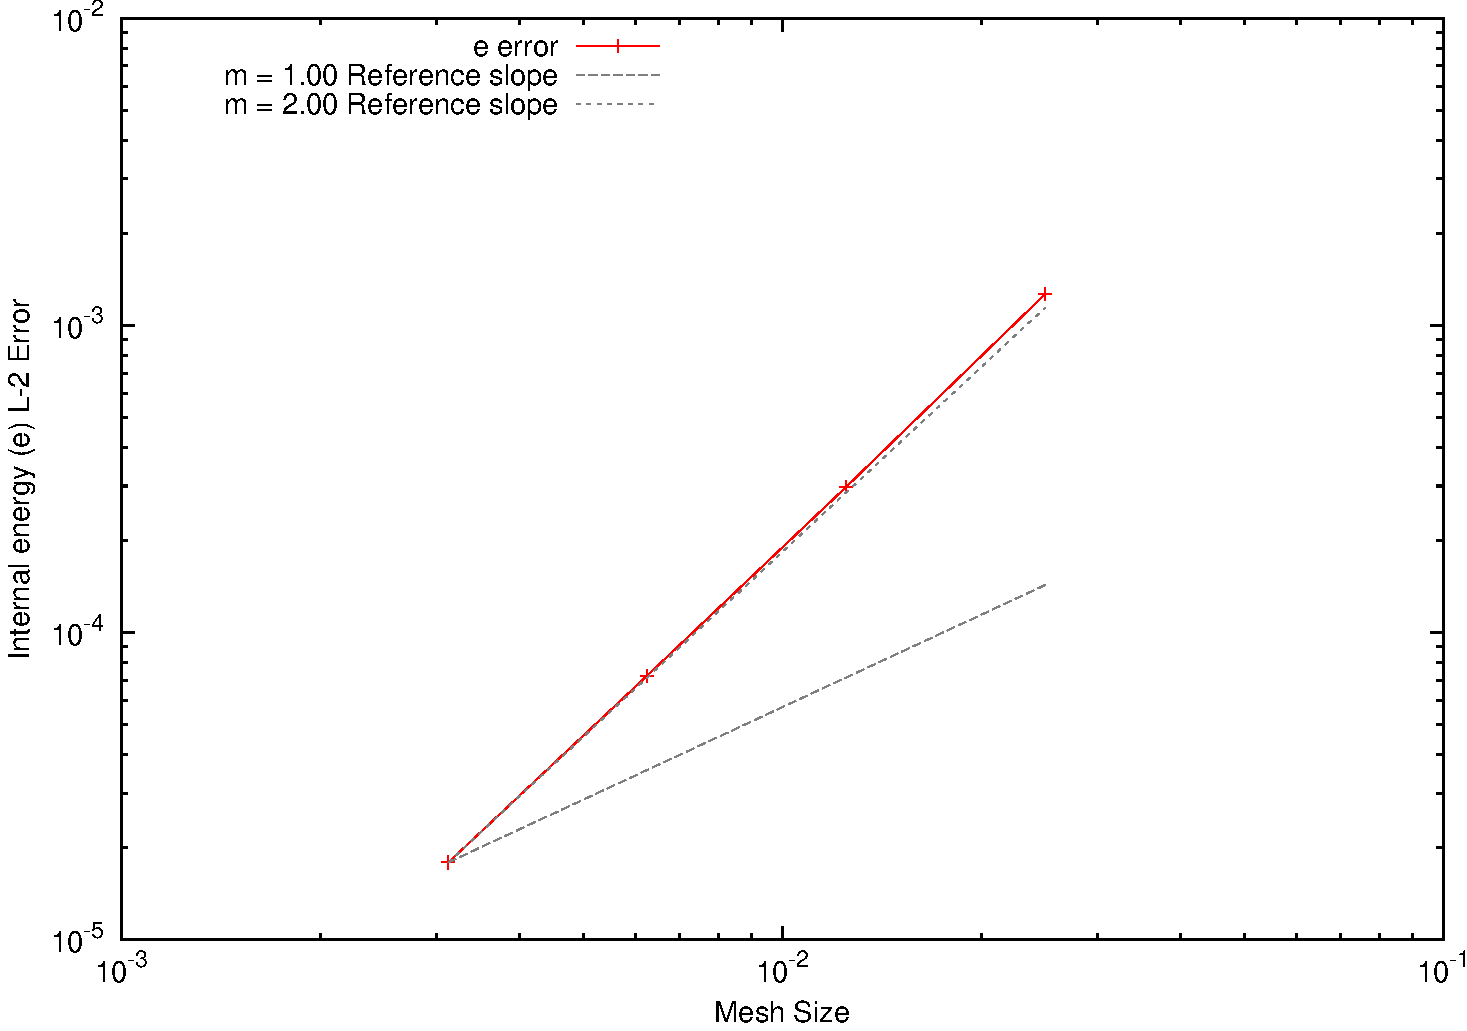
\includegraphics[width=0.99\linewidth]{convergence_plot/e_convergence.pdf}
    \caption{\label{e_convergence} MMS Spatial Convergence}
\end{subfigure}
\end{figure}
%    \vspace{0.7em}
%    \vspace{0.7em}
%    \centering \textbf{Problem 2:} Optically thin (left) and thick (right) regions
%    \vspace{0.7em}
%\begin{figure}
%\begin{subfigure}{0.49\textwidth}
%    \centering
%    \includegraphics[width=0.99\textwidth]{two_mat_conv.pdf}
%    \caption{Spatial mesh convergence.\label{twomat_full}}
%\end{subfigure} 
%\begin{subfigure}{0.49\textwidth}
%\centering
%    \includegraphics[width=0.99\textwidth]{two_mat_ho_compare.pdf}
%    \caption{\colb{ECMC} vs \colr{Standard MC} as HO solver \label{twomat_quick}}
%\end{subfigure}
%\end{figure}

\end{block}
\vfill
%%%%%%%%%%%%%%%%%%%%%%%%%%%%%%%%%%%%%%%%%%%%%%%%%%%%%%%%%%%%%%%%%%%%%%%%%%%
    \begin{block}{Conclusions}
    \begin{itemize}
        \item We are able to produce accurate radiative shock solutions.
        \item We demonstrated second-order accuracy for a smooth manufactured solution. 
      \end{itemize}
    \end{block}
     \vfill
    %%%%%%%%%%%%%%%%%%%%%%%%%%%%%%%%%%%%%%%%%%%%%%%%%
}
\end{minipage}
\end{beamercolorbox}
\end{column}

\end{columns}
\end{frame}
\end{document} 
         
         
 
         
         
  
